\section{Durchführung}
\label{sec:Durchführung}

Der Versuchsaufbau ist in Abbildung \ref{fig:roent} dargestellt.
\begin{figure}
    \centering
    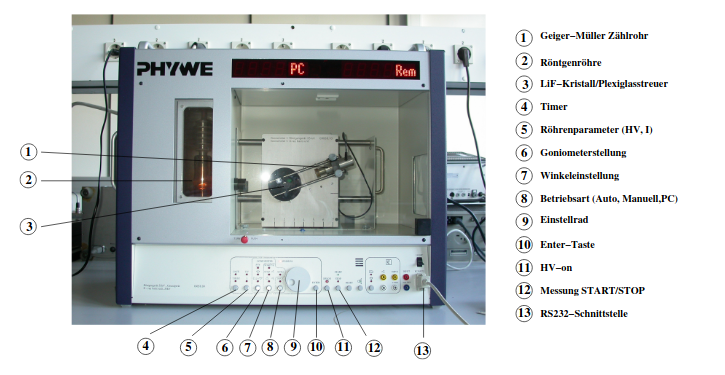
\includegraphics[width=\textwidth]{Röntgenröhre.png}
    \caption{Röntgenröhre}
    \label{fig:roent}
\end{figure}
Links (2) ist eine Kupfer-Röntgenröhre verbaut, die Röntgenstrahlung auf einen LiF-Kristall bzw.
einen Plexiglas-Streuer (3) aussendet. An diesem ist das Geiger-Müllerzählrohr (1) befestigt. \\
Zunächst wird das Emmisionsspektrum der Beugungsordnung n=1 aufgenommen. Hierzu wird eine 2 mm 
Blende und der LiF-Kristall verwendet. \\
Im nächsten Schritt wird die Transmission des Aluminium-Absorbers gemessen. Dazu wird eine
Aluminiumplatte vor der 2 mm Blende installiert. Damit man 
den Einfluss der Aluminiumplatte richtig einschätzen kann, wird auch eine Messung ohne 
die Platte durchgeführt. Außerdem muss zur Korrektur des durch die Totzeit des Geiger-
Müllerzählrohrs entstandenen Fehlers die Rechnung
\begin{equation}
    I = \dfrac{N}{1-\tau \cdot N}
\end{equation}
durchgeführt werden. \\
Nun soll die Intensität $I_0$ der Cu-Röhre bestimmt werden. Zu diesem Zweck wird der Plexiglasstreuer,
durch den der LiF-Kristall nun ersetzt wird, auf 45 und das Geiger-Müllerzählrohr auf 90 Grad 
eingestellt.
\begin{figure}
    \centering
    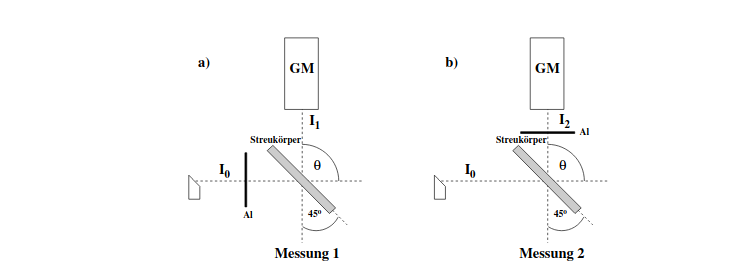
\includegraphics[width=\textwidth]{Experimenteller Aufbau.png}
    \caption{Experimenteller Aufbau}
    \label{fig:exau}
\end{figure}
Im Folgenden wird nun wie in Abbildung \ref{fig:exau} dargelstellt, der Aluminiumabsorber einmal in 
den Strahlengang zwischen Röntgenröhre und Streukörper und einmal in den Strahlengang
zwischen Streukörper und Geiger-Müllerzählrohr gebracht und die Transmission $T_1=\dfrac{I_1}{I_0}$
bestimmt. 


